\documentclass[a4paper]{article}

\usepackage[T1]{fontenc}              % Codificação para português 
\usepackage[brazilian]{babel}         % Português
\usepackage{hyphenat}                 % Use hifens corretamente
\usepackage{hyperref}                 % Links para páginas web
\usepackage{graphicx}                 % Figuras
\usepackage{float}                    % Figuras no lugar "esperado"
\graphicspath{{./images/}}            % Localização das imagens
\usepackage{fancyhdr}                 % Header estilo DCC
\setlength{\headheight}{24pt}

\title{Trabalho Prático II}
\author{Igor Lacerda Faria da Silva}
\date{\href{mailto:igorlfs@ufmg.br}{\texttt{igorlfs@ufmg.br}} }

\begin{document}

\pagestyle{fancy}
\lhead{Prof. Adriano Veloso

	Aprendizado de Máquina}
\rhead{DCC / ICEx / UFMG

	2023.1}

\maketitle

\section*{Introdução}
\label{sec:Introdução}

O objetivo deste trabalho é aprofundar o conhecimento do algoritmo de \textit{boosting}, implementando-o “do zero”. Mais especificamente, foi implementado o \textit{AdaBoost} com \textit{stumps} (árvores de decisão com apenas um nó). Como exemplo, foi analisado o \textit{dataset} \href{https://archive.ics.uci.edu/dataset/101/tic+tac+toe+endgame}{\texttt{Tic-Tac-Toe Endgame}}, que contém todos as instâncias de “Jogo da Velha” em que o jogador inicial é $x$, além do resultado do jogo. No entanto, o programa é robusto: é possível usar outros bancos de dados apenas trocando alguns parâmetros.

Foi usada validação cruzada (\textit{5-fold}) para avaliar o desempenho do modelo. Este relatório apresenta a evolução do erro variando-se a quantidade de \textit{stumps}.

\section*{Desenvolvimento}%
\label{sec:Desenvolvimento}

\begin{figure}[H]
	\begin{center}
		{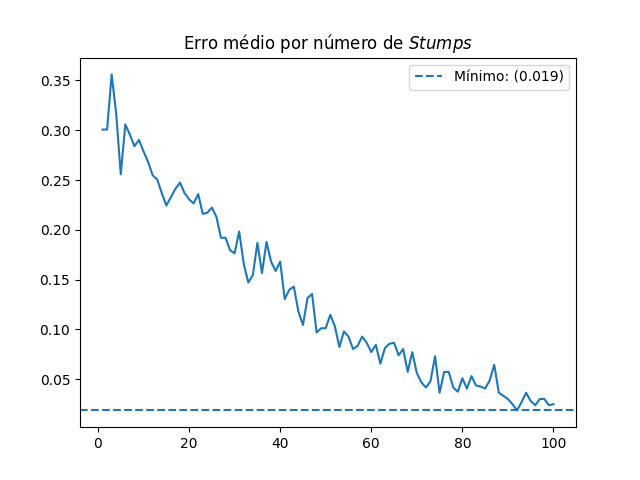
\includegraphics[height=7cm]{./images/error_per_stumps.png}}
	\end{center}
	\caption{Erro pelo número de \textit{stumps}, na validação cruzada. \label{fig:aeh}}
\end{figure}

O desempenho do modelo, de forma geral, não foi satisfatório. É incomum que alguma divisão da validação cruzada atinga a “barreira” de 20\% de erro, e a média raramente fica abaixo de 25\%. É possível perceber uma melhora no desempenho, conforme são adicionados mais \textit{stumps}, mas a partir de cerca de 20 \textit{stumps}, o desempenho piora drasticamente. Presumivelmente isso acontece porque são adicionados vários \textit{stumps} da mesma classe, o que tende a degradar o modelo.

\end{document}
